Let's consider the \textbf{momentum equation} in its \textbf{Eulerian form}:
\[
\frac{\partial {\bf u}}{\partial t} + ({\bf u} \cdot \nabla){\bf u} = -\frac{\nabla p}{\rho} + {\bf f}_{\rm ext}.
\]
Now, one question we might ask is if there are any dynamical \textbf{first integrals} which can be obtained from physical arguments. In general, this is not an easy undertaking; however, when the flow \textbf{is steady}, it can be shown to have a first integral in the form of \textbf{Bernoulli's Theorem}.
\par
In order to construct this first integral, we want to effectively construct a \textbf{potential} for the entire flow which behaves analogously to that of gravitation or electrodynamics. Unfortunately, not all of the terms in the Euler equation are easily cast as gradients of scalar potentials. Consider the pressure term:
 Consider the pressure term:
\[
-\frac{\nabla p}{\rho} = -\nabla h(\rho),
\]
for some $h$. The equestion becomes what exactly $h$ is. Formally, we have
\[
\frac{-\nabla p}{\rho} = - \frac{1}{\rho}\frac{dp}{d\rho} \nabla \rho = - \nabla h(p).
\]
If we integrate, we have
\[
dh = \frac{1}{\rho} \frac{dp}{d\rho} d\rho = \frac{dp}{\rho} \implies h(p) = \int^p \frac{dp}{\rho}.
\]
This $h$ has a name: it is the \textbf{specific enthalpy of the material}. 

Our equation has therefore taken the form
\[
\frac{\partial {\bf u}}{\partial t} + ({\bf u} \cdot \nabla){\bf u}  = -\nabla h+ {\bf f}_{\rm ext}.
\]
Now, it can be shown that (vector identity),
\[
({\bf A} \cdot \nabla){\bf A} = \frac{1}{2}\nabla(|{\bf A}|^2) - {\bf A} \times (\nabla \times {\bf A}).
\]
As such, we may write the second term on the LHS as
\[
({\bf u \cdot \nabla}){\bf u}  = \frac{1}{2}\nabla(u^2) - {\bf u} \times (\nabla \times {\bf u}).
\]
\par
\textbf{What have we gained?} Here's the idea, we now have almost entirely gradient operators in the Euler equation, except for this rather odd looking curl term. Recalling from definition~\ref{def:vorticity} that
the \textbf{vorticity of flow} is
\[
\boldsymbol{\omega} = \nabla \times {\bf u},
\]
we may write Euler's equation in the form
\[
\boxed{
\frac{\partial {\bf u}}{\partial t} +\nabla\left(\frac{1}{2}u^2 + h + \phi\right) = {\bf u} \times \boldsymbol{\omega}.}
\]
It is from this expression that we can begin to elucidate \textbf{Bernoulli's Theorem}.


\section{Bernoulli's Theorem}

The expression above is already the \textbf{most general} form of the famous \textbf{Bernoulli's Theorem}, which we now state in full clarity:

\vspace{0.5cm}
\begin{theorem}[Bernoulli's Theorem]
For \textbf{any fluid flow} in which the \textbf{only external forces} are those derived from potentials, \textbf{Bernoulli's Theorem} states that
\begin{equation}
    \label{eq:bernoulli-general}
    \frac{\partial {\bf u}}{\partial t} 
    + \nabla\left(\frac{1}{2}u^2 + \Phi\right) 
    + \frac{\nabla P}{\rho} 
    = {\bf u} \times \boldsymbol{\omega}.
\end{equation}
Here, $\Phi$ is the external potential, $\rho$ is the mass density, $P$ is the pressure, and $\boldsymbol{\omega} = \nabla \times \mathbf{u}$ is the vorticity. 
\end{theorem}
\vspace{0.5cm}

This form is exact and general, but not always directly useful in applications. The power of Bernoulli’s theorem lies in its \textbf{corollaries}, which arise under additional assumptions that simplify the dynamics.

\subsection{First Corollary: Steady Barotropic Flow}

Our first corollary concerns barotropic flows which are in a steady state:
\vspace{0.5cm}
\begin{corollary}
Consider a fluid which is in \textbf{steady-state} ($\partial_t {\bf u} = 0$), and which follows a \textbf{barotropic equation of state}, i.e.\ $P = P(\rho)$. If the only external forces are those derived from potentials (combining to form $\Phi$), then the flow obeys
\begin{equation}
    \label{eq:bernoulli-steady}
    {\bf u} \cdot \nabla \mathcal{B} = 0,
\end{equation}
where $\mathcal{B}$, the \textbf{Bernoulli function}, is given by
\[
\mathcal{B} = \frac{1}{2}u^2 + h + \Phi,
\]
and $h$ is the \textbf{specific enthalpy}, defined by
\[
h(\rho) = \int^\rho \frac{dP}{\rho'}.
\]
\end{corollary}

\begin{proof}
In steady flow the time derivative vanishes. Under the barotropic assumption,
\[
\frac{\nabla P}{\rho} = \nabla h.
\]
Substituting into \eqref{eq:bernoulli-general} gives
\[
{\bf u} \cdot \nabla \left( \tfrac{1}{2}u^2 + h + \Phi \right) = 0,
\]
which is precisely \eqref{eq:bernoulli-steady}.
\end{proof}
\vspace{0.5cm}

Equation \eqref{eq:bernoulli-steady} shows that the Bernoulli function $\mathcal{B}$ is \textbf{constant along streamlines}. That is, as one moves with the flow, the combination of kinetic energy, enthalpy, and potential energy remains conserved. This conservation law is a cornerstone of fluid dynamics, forming the basis for practical applications ranging from aerodynamics (lift and pressure differences) to astrophysical accretion flows.

\subsection{Second Corollary: Irrotational Flow}

We may also make refinements to the Bernoulli Theorem when we have \textbf{irrotational flow}:
\vspace{0.5cm}
\begin{corollary}
If the flow is \textbf{irrotational}, i.e.\ $\boldsymbol{\omega} = 0$, then the velocity field can be written as the gradient of a scalar potential:
\[
\mathbf{u} = \nabla \psi.
\]
In this case, Bernoulli’s theorem reduces to the statement that
\[
\nabla\left(\frac{\partial \psi}{\partial t} + \mathcal{B}\right) = 0.
\]
Equivalently,
\[
\frac{\partial \psi}{\partial t} + \frac{1}{2}u^2 + h + \Phi = f(t),
\]
where $f(t)$ is a function of time alone. This is the most general form of Bernoulli’s theorem for irrotational flow.
\end{corollary}
\begin{proof}
If $\boldsymbol{\omega} = 0$, then $\mathbf{u}$ is curl-free and may be expressed as the gradient of a velocity potential $\psi$. Substituting $\mathbf{u} = \nabla \psi$ into \eqref{eq:bernoulli-general} yields
\[
\nabla\!\left(\frac{\partial \psi}{\partial t} + \frac{1}{2}u^2 + h + \Phi \right) = 0,
\]
which implies that the quantity in parentheses must be spatially uniform, though it may still vary in time. Hence the stated result.
\end{proof}
\vspace{0.5cm}
The introduction of a velocity potential is a profound simplification: the vector equation of motion for the fluid is reduced to a scalar relation. Even in unsteady situations, the dynamics can be reformulated in terms of $\psi$, which greatly facilitates both analysis and computation. This scalar Bernoulli equation is the foundation of potential flow theory, allowing one to analyze flows with far less complexity than in the general rotational case.

\subsection{Third Corollary: Steady Irrotational Flow}

The final corollary worth mentioning is a refinement of the previous one in which we now also have a steady flow:
\vspace{0.5cm}
\begin{corollary}
If the flow is both \textbf{steady} and \textbf{irrotational}, then the Bernoulli function
\[
\mathcal{B} = \frac{1}{2}u^2 + h + \Phi
\]
is not only conserved along streamlines, but is in fact \textbf{constant throughout the entire flow domain and independent of time}.
\end{corollary}

\begin{proof}
In steady flow, $\partial_t \psi = 0$, so the unsteady Bernoulli relation of the previous corollary reduces immediately to
\[
\frac{1}{2}u^2 + h + \Phi = \text{constant}.
\]
This constant holds everywhere in the flow, not just along streamlines.
\end{proof}
\vspace{0.5cm}

This is the most celebrated and practically useful form of Bernoulli’s theorem. It asserts that in steady, irrotational, barotropic flow under conservative forces, every fluid element shares the same Bernoulli constant. Physically, it represents the conservation of mechanical energy per unit mass — the sum of kinetic energy, enthalpy, and potential energy — across the entire flow field. This global constraint underlies classical results in aerodynamics (such as lift and pressure distribution), hydrodynamics (water jets, weirs, and pipe flow), and astrophysics (stellar winds and accretion flows). It is this version of Bernoulli’s theorem that most clearly illustrates the intimate link between fluid kinematics and conservation of energy.

\begin{bigidea}
\textbf{Bernoulli’s Theorem} is a reformulation of Euler’s equations that reveals a powerful energy conservation principle in fluid flows. Its critical insights are:

\begin{itemize}
  \item In its \textbf{general form}, the theorem is equivalent to the Euler equations, with an explicit vorticity term that prevents a simple conservation law.
  \item Under the assumptions of \textbf{steady, barotropic flow}, the \textbf{Bernoulli function}
  \[
  \mathcal{B} = \tfrac{1}{2}u^2 + h + \Phi
  \]
  is conserved \emph{along streamlines}, representing the conservation of mechanical energy per unit mass (kinetic + enthalpy + potential).
  \item If the flow is further \textbf{irrotational}, then a velocity potential $\psi$ exists and Bernoulli’s theorem reduces to a scalar relation. In this case, $\mathcal{B}$ is spatially uniform at each instant.
  \item In the most restrictive case of \textbf{steady, irrotational flow}, $\mathcal{B}$ is globally constant throughout the domain and independent of time — the classic textbook form of Bernoulli’s law.
\end{itemize}

\noindent \textbf{Takeaway:} The hierarchy of Bernoulli results reflects progressively stronger assumptions: from a general Eulerian identity, to conservation along streamlines, to global constancy in potential flows. This framework underpins the use of Bernoulli’s equation in engineering, aerodynamics, and astrophysics.
\end{bigidea}


\section{Vorticity and Kelvin's Circulation Theorem}

Some more is worth saying on the subject of \textbf{vorticity}. In a general flow, where the requirements of irrotational flow and steady flow have been removed, we still have a \textbf{momentum equation} in the form
\[
\frac{\partial {\bf u}}{\partial t} = - \nabla \mathcal{B} + {\bf u} \times \boldsymbol{\omega}.
\]
From this result, we may arrive at the very useful \textbf{Helmholtz's Theorem}:
\vspace{0.6 cm}
\begin{theorem}[Helmholtz's Theorem]
For any fluid which is \textbf{irrotational} at a time $t_0$, then for any prior or later time $t$, the fluid must remain irrotational unless viscous forces are at play.
\end{theorem}
\begin{proof}
    If we take the curl of both sides of the equation above, we find
    \[
    \frac{\partial \boldsymbol{\omega}}{\partial t} = - \nabla \times \nabla \mathcal{B} + \nabla \times ({\bf u} \times \boldsymbol{\omega}).
    \]
    Relying on the fact that the curl of a gradient is 0, we have
    \[
    \frac{\partial \boldsymbol{\omega}}{\partial t} = \nabla \times ({\bf u} \times \boldsymbol{\omega}).
    \]
    As such, if $\boldsymbol{\omega} = 0$, then it cannot evolve in time.
\end{proof}
\vspace{0.6cm}
We can actually take this concept even further. Formally, consider a \textbf{simple-closed contour (loop)} in the flow $(\partial S(t))$. \rmk{You can think if this as a set of fluid elements at time $t_0$ which form a contour and then evolve with the flow from there, defining the contour in time.} Now, that contour will (of course), define a surface and the \textbf{vorticity flux} across that contour is
\[
F = \int_{S(t)} \boldsymbol{\omega} \cdot d{\bf S}. 
\]
We might ask how this evolves as the fluid moves with time. The \textbf{Lagrangian Derivative} will be required to incorporate the change in the vorticity, but also the change in the contour as well. We can define an equivalent quantity to $F$: the \textbf{circulation} around the contour. By Stoke's theorem,
\[
\Gamma = \int_S (\nabla \times  {\bf u}) \cdot d{\bf S} = \oint_{\partial S} {\bf u} \cdot d{\bf l}. 
\]
Now, let's parameterize the \textbf{lagrangian configuration} of the boundary as $\alpha \in [0,1]$ such that
\[
d{\bf l} = \partial_\alpha {\bf X} d\alpha.
\]
the change in the circulation with time is then
\[
\frac{D\Gamma}{Dt} = \frac{d}{dt} \int_0^1 d\alpha {\bf u}({\bf X},t) \cdot \partial_\alpha {\bf X}.
\]
Pulling the time derivative in, we have
\[
\frac{D\Gamma}{Dt} = \int_0^1 \frac{D{\bf u}}{Dt} \cdot \partial_\alpha {\bf X} + {\bf u} \cdot \partial_\alpha\frac{D{\bf X}}{Dt} \; d\alpha
\]
Now, $D{\bf X}/Dt = {\bf u}({\bf X},t)$, so that second term has the form
\[
\int_0^1 ({\bf u} \cdot \partial_\alpha){\bf u} \;d\alpha = \int_0^1 {\bf (u \cdot \nabla){\bf u} \cdot \partial_\alpha {\bf X}}\; d\alpha
\]
Now, if we expand the $D{\bf u}/Dt$, term as well, it cancels with this term above and we get
\[
\frac{D\Gamma}{Dt} = \oint \frac{D{\bf u}}{Dt} \cdot d{\bf l}.
\]
If we now apply the \textbf{Euler Equation} in the special case where \textbf{Bernoulli's theorem holds}, then this RHS is a potential and therefore has no circulation. This implies \textbf{Kelvin's Circulation Theorem}, which claims that 
\[
\frac{D\Gamma}{Dt} = 0.
\]

\section{Aside: Potential Flow}

A worthwhile note at this stage is the following: if we have an \textbf{irrotational fluid}, then there exists some $\psi$ such that
\[
{\bf u}({\bf x},t) = \nabla \psi({\bf x},t).
\]
This occurs because ${\bf u}$ has no curl if it is irrotational. Additionally, if we have a \textbf{incompressible fluid}, then
\[
\nabla \cdot {\bf u} = 0 \implies \nabla^2 \psi = 0.
\]
As such, these flow problems are solved via the \textbf{Laplace equation}.

\section{DeLaval's Nozzle}

Consider the following very basic problem:
\begin{center}
\textit{A pipe of cross sectional area $A(z)$ carries a steady flow with variables $u(z)$, $\rho(z)$, and $p(z)$. Determine the relationship between each of these and the cross sectional area.}
\end{center}

Now, in this scenario, we will \textbf{ignore gravity} and instead treat the simpler problem of a gas in a pipe and its relevant velocity and pressure. We'll likewise assume a \textbf{barotropic equation of state} as we have done in many previous scenarios.
\par
Since the flow is \textbf{steady}, we cannot allow mass to build up anywhere. This gives us our first piece of information. We know then that
\[
\rho u A = \rm{constant.}
\]
Now, the Euler equation for momentum tells us that
\[
\frac{D{\bf u}}{Dt} = (u\cdot\nabla)u = - \frac{dp}{d\rho} d\log \rho.
\]
From mass conservation, we have
\[
\log \rho + \log u + \log A = C \implies d\log \rho = - d\log u - d\log A.
\]
We can thus write
\[
\frac{-dp}{d\rho} d\log \rho = \frac{dp}{d\rho}\left[d\log u + d\log A\right] = c_s^2[d\log u + d\log A].
\]
Now, this is where we make our \textbf{tricky simplification}: we assume that the flow is \textbf{irrotational} (a valid assumption), and so
\[
({\bf u} \cdot \nabla){\bf u} = \frac{1}{2}\nabla u^2 - {\bf u} \times \boldsymbol{\omega} = \frac{1}{2}\nabla u^2.
\]
This can be written as $u \nabla u = u^2 \nabla \log u$, so
\[
\boxed{
(u^2-c_s^2) d\log u = c_s^2 d\log A
}
\]
\begin{remark}
    You can play around with this mentally quite a bit. Let's consider some scenarios where $u$ starts out subsonic so that we have $- d\log u \sim d\log A$. 
    \begin{itemize}
        \item As we \textbf{contract the nozzle}, we \textbf{increase velocity}, but it requires more and more contraction as we get closer to $c_s$. we \textbf{cannot make a sonic transition} until the nozzle reverts.
    \end{itemize}

If we are \textbf{supersonic}, then we instead need $d\log A \sim d\log u$, so the nozzle expands to move our fluid faster. This is the idea behind which rocket engines build their jets. We start with a thermal energy rich fluid with low velocity. As it moves down the nozzle, it speeds up until the center, when the nozzle starts expanding again, the speed goes super-sonic and a lot of that thermal energy is converted to kinetic energy. This is a \textbf{very effective way to convert thermal to mechanical energy}.
\end{remark}
The De Laval Nozzle can be used to partially describe the nature of astrophysical jets; however, other (magnetohydrodynamical) effects are relevant in these scenarios.

\section{Bondi Accretion}

\textbf{Bondi accretion} is the simplest classical model of accretion in a spherically symmetric system. It relies on several significant assumptions and derives the relevant hydrodynamic behavior of the system. In this section, we will perform the derivation and cite the relevant limitations.

\subsection{The Intuitive Picture}

The full hydrodynamic derivation of Bondi accretion is rigorous but not something one
needs to memorize. What is most useful to retain is the simple physical intuition that
leads directly to the correct scaling for the accretion rate.

\par
The key concept is the existence of an \textbf{accretion radius}, $r_{\rm acc}$, where
the gravitational binding energy of the accretor balances the thermal energy of the gas:
\[
\frac{GM}{r_{\rm acc}} \sim c_s^2(\infty).
\]
Inside this radius, gravity dominates over pressure support, and gas is effectively
captured. Thus $r_{\rm acc} \sim GM/c_s^2(\infty)$ defines the size of the accretor's
sphere of influence.

\par
Now, how much material is drawn in? Imagine that gas within this radius is funneled
inward at roughly the sound speed, $c_s(\infty)$, since this is the characteristic
velocity scale of the medium. The \emph{feeding rate} of mass across the surface of
the capture sphere is then
\[
\dot{M} \sim \rho_\infty \, v \, A
\;\;\;\;\;\; \sim \;\;\;\; \rho_\infty \, c_s(\infty) \, \pi r_{\rm acc}^2.
\]

\par
Substituting the scaling for $r_{\rm acc}$,
\[
\dot{M} \;\sim\; \pi \rho_\infty \left(\frac{GM}{c_s^2(\infty)}\right)^2 c_s(\infty).
\]

\par
Thus we immediately arrive at the Bondi scaling
\[
\boxed{\dot{M} \;\propto\; \frac{(GM)^2 \rho_\infty}{c_s^3(\infty)}.}
\]

\par
This heuristic argument is not exact—it ignores the subtleties of transonic flow and
the precise dependence on the polytropic index $\gamma$—but it captures the correct
dependence on $M$, $\rho_\infty$, and $c_s$. The rigorous hydrodynamic treatment
merely supplies the order-unity prefactor. The essential physics is therefore
straightforward: accretion is controlled by the size of the gravitational capture
region and by the rate at which gas can flow into it at the ambient sound speed.

\subsection*{Assumptions}

In Bondi accretion, we make the following simplifying assumptions:
\vspace{0.5cm}
\begin{enumerate}
    \item \textbf{Spherical symmetry: }The entire flow is treated as spherically symmetric and the accretor is at rest relative to the ambient material. \rmk{This plays out mathematically immediately.}
    \item \textbf{Steady State}: The nature of the flow does not change over time. Formally, this means that any of the field variables $\psi$ is independent of time. \rmk{This is a trickier requirement as it allows us to define a constant accretion rate; however, we know this to be not in keeping with physical systems.}
    \item \textbf{Polytropic Equation of State}: We assume a \textit{barotropic equation of state} following the form of a polytrope
    \[
    P = \kappa \rho^\gamma.
    \]
    \rmk{In the limiting cases, we have either adiabatic flows (optically thin) or isothermal (optically thick).}
    \item \textbf{Gravity}: Is assumed to be fully Newtonian and the accretor is treated as a point mass.
    \item \textbf{No Additional Forces}: The only relevant force is that of gravity. MHD effects are ignored.
\end{enumerate}

\subsection*{Derivation}

Formally, we have 3 equations: the \textbf{continuity equation}, the \textbf{Euler equation}, and the \textbf{equation of state}. In this scenario, continuity provides that
\[
\underbrace{\frac{\partial \rho}{\partial t}}_{\text{$=0$ (assumpt. 2)}} + \nabla \cdot(\rho{\bf u}) = 0 \implies \frac{1}{r^2} \partial_r[r^2 \rho {\bf u}] = 0.
\]
We therefore find that
\[
r^2 \rho {\bf u} = \rm{Constant}.
\]
This is a very useful integral of the motion because the accretion rate is
\[
\dot{M} = -4\pi r^2 \rho u = {\rm Constant}.
\]
\rmk{This is deducible from the fact that we have steady flow and therefore cannot collect mass in shells.}
\par
We also have the \textbf{Euler Equation} in the form
\[
u \frac{du}{dr} + \frac{1}{\rho}\frac{dP}{dr} + \frac{GM}{r^2} = 0.
\]
Using the polytropic equation of state,
\[
\frac{dP}{dr} = \frac{dP}{d\rho} \frac{d\rho}{dr} = c_s^2 \frac{d\rho}{dr}.
\]
\rmk{Remember that $c_s^2$ is a function of radius.} From the continuity equation,
\[
\frac{1}{r^2} \partial_r (\rho r^2 u) = 0 \implies \underbrace{\rho \frac{1}{r^2}\partial(r^2u) + u \partial_r \rho}_{\text{product rule}} = 0 \implies \partial_r \log \rho = - \frac{1}{r^2 u} \partial_r ur^2,
\]
so (\rmk{substitute $\partial_r \log \rho$ and then expand out the prod. rule}),
\[
u \frac{du}{dr} - \frac{c_s^2}{ur^2} \frac{du}{dr} + \frac{GM}{r^2} = 0.
\]
If we perform some rearrangements, we find the critical equation which will consume our discussion for the rest of the section:
\begin{equation}
    \boxed{
    \frac{1}{2}\left(1-\frac{c_s^2}{u^2}\right) \frac{du^2}{dr} = -\frac{GM}{r^2} \left[1-\frac{2c_s^2 r}{GM}\right].
    }
\end{equation}

\subsubsection{The Sonic Point}
\begin{figure}
    \centering
    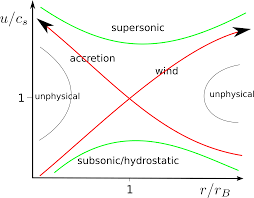
\includegraphics[width=0.75\linewidth]{Pictures/figures/bondi_regime.png}
    \caption{The parameter space of Bondi-accretion solutions. The sonic point $r_b$ is shown on the $x$-axis and the velocity on the $y$ axis.}
    \label{fig:bondi_regime}
\end{figure}
It is not immediately clear why we should have gone to all the work of building out this complicated ODE for ourselves; however, we can see that there are several very interesting features. The most important of these is that equation~\eqref{eq:bondi_critical_radius} is \textbf{singular} at 
\begin{equation}
    \label{eq:bondi_critical_radius}
    \boxed{
    r_s = \frac{GM}{2c_s^2}.
    }
\end{equation}
\rmk{Remember that $c_s$ is still a function of the radius. This means that this is \textbf{implicit}.} This is the so-called \textbf{sonic point} of the flow: \textit{if} the flow is going to make a transition to or from \textbf{sub-sonic} to \textbf{super-sonic}, it \textit{must occur at $r_s$.} This means that there are 4 important regimes to consider:
\vspace{0.5cm}
\begin{enumerate}
    \item \textbf{Transitioning Solution}: If we enforce that $u = c_s$ at the sonic radius, then the solution is entirely determined by the choice of behavior as $r\to \infty$ or by the choice of behavior as $r\to0$. If we let $u \to 0$ at $\infty$, then we obtain \textbf{accreting flows} featuring a transition point, and if we permit $u \to 0$ as $r\to 0$, then we obtain \textbf{wind flows} with transition points.
    \item \textbf{Non-Transitioning Solutions}: If a solution is not going to have $u=c_s$, then one \textit{must let $du^2/dr = 0$} at the sonic radius. In this case, the entire solution is fixed either by the behavior at either asymptote or by the behavior (the velocity) at the sonic point.
\end{enumerate}
\vspace{0.5cm}

\subsubsection{Bernoulli Flow}
We have now clarified the general behavior of the ODE we wish to solve and identified the relevant regimes. Most importantly, we are now able to recognize that uniqueness of our solution can be guaranteed by specifying the behavior both at the critical point and at $\infty$. Let us now fully solve the problem. To do so, we will apply \textbf{Bernoulli's Theorem}:
\[
u \frac{du}{dr}+ \nabla(h+\phi) = 0 \implies \frac{1}{2} u^2 + h + \phi = 0.
\]
For a \textbf{barotropic equation of state}, the specific enthalpy is
\[
h = \int \frac{dP}{\rho} = \int \frac{dP}{d\rho} \frac{1}{\rho} d\rho = \frac{K\gamma}{\gamma -1} \rho^{\gamma - 1} = \frac{c_s^2}{\gamma -1}.
\]
Thus,
\begin{equation}
    \frac{u^2}{2} + \frac{c_s^2}{\gamma -1} - \frac{GM}{r} = \rm{Constant}.
\end{equation}
\rmk{In the isothermal case, we actually need to have a logarithm here instead of $\gamma -1$.}
\par
Now, for \textbf{accreting flows}, we have $u(\infty) = 0$. Thus,
\[
c_s^2(\infty) = C(\gamma-1) \implies C = \frac{c_s^2(\infty)}{\gamma -1}.
\]
Additionally, the sonic point requires that
\[
c_s^2(r_s) = \frac{GM}{2r_s},
\]
so at $r_s$, we have
\[
\frac{c_s^2(r_s)}{2} + \frac{c_s^2(r_s)}{\gamma -1} - 2c_s^2(r_s) = \frac{c_s^2(\infty)}{\gamma -1}.
\]
So
\begin{equation}
\boxed{\
    c_s(r_s) = c_s(\infty) \left(\frac{2}{5 - 3\gamma}\right)^{1/2}
    }
\end{equation}
\rmk{Once again, we see that $\gamma = 5/3$ is not permitted! In practical scenarios, we are never really ideal, so this is fine, but nonetheless, it is worth noting.}
The mass accretion rate is constant at all radii, so we can evaluate it at the sonic point and find
\begin{equation}
    \boxed{
    \dot{M} = \pi G^2 M^2 \frac{\rho(\infty)}{c_s^3(\infty)} \left[\frac{2}{5-3\gamma}\right]^{(5-3\gamma)/2(\gamma-1)}.
    }
\end{equation}
\subsubsection{The Accretion Radius}

The Bondi solution motivates the introduction of a characteristic length scale, the
\textbf{accretion radius}, defined as
\begin{equation}
    \label{eq:bondi_radius}
    r_{\rm acc} \equiv \frac{2GM}{c_s^2(\infty)}.
\end{equation}
This can be understood from a simple energetic argument. At radius $r$, the
\textbf{gravitational binding energy per unit mass} is
\[
E_{\rm grav} \sim \frac{GM}{r},
\]
while the \textbf{thermal energy per unit mass} of the gas is set by the sound speed,
\[
E_{\rm th} \sim c_s^2(\infty).
\]
The radius $r_{\rm acc}$ is defined as the point where these two energy scales balance:
inside this radius, gravitational attraction dominates over thermal motions, so gas is
gravitationally captured by the accretor. Outside this radius, pressure forces can
support the gas against collapse. Thus, $r_{\rm acc}$ plays the role of an effective
``sphere of influence'' for accretion.

\begin{remark}
Note that $r_{\rm acc}$ is distinct from the precise sonic radius $r_s$, which depends
on the local sound speed $c_s(r_s)$. The accretion radius is defined in terms of the
\emph{asymptotic} sound speed at infinity, and provides a more intuitive, order-of-magnitude
measure of the capture region.
\end{remark}

\subsubsection{Free-Fall Behavior Beyond the Sonic Point}

Once the gas passes through the sonic point, the flow is \textbf{supersonic}. In this
regime, pressure forces are negligible compared to inertia and gravity: the gas
effectively undergoes free fall. This allows us to extract the asymptotic scaling of
velocity, density, and temperature in the inner region.

\paragraph{Velocity:} In free fall onto a point mass, the velocity is set by the
gravitational potential:
\[
u(r) \sim \left(\frac{2GM}{r}\right)^{1/2}.
\]

\paragraph{Density:} The accretion rate is constant at all radii,
\[
\dot{M} = 4\pi r^2 \rho u.
\]
Substituting the free-fall velocity,
\[
\rho(r) \sim \frac{\dot{M}}{4\pi r^2 u(r)} \;\propto\; r^{-3/2}.
\]

\paragraph{Temperature:} For a polytropic gas,
\[
T \propto \frac{P}{\rho} \propto \rho^{\gamma-1}.
\]
Thus, in the inner free-fall region,
\[
T(r) \;\propto\; r^{-3(\gamma-1)/2}.
\]
For example:
\begin{itemize}
    \item Isothermal case ($\gamma=1$): $T(r) = \rm{const}$.  
    \item Adiabatic monoatomic gas ($\gamma=5/3$): $T(r) \propto r^{-1}$.
\end{itemize}


\subsection*{Summary and Key Formulae}

Bondi accretion provides the simplest classical model for spherically symmetric accretion onto a compact object. While highly idealized, it illustrates several key physical principles:

\begin{itemize}
    \item The flow is uniquely determined by the requirement that it pass smoothly through the \textbf{sonic point}. This makes the solution transonic, subsonic at infinity and supersonic near the accretor. 
    \item The \textbf{accretion radius} 
    \[
    r_{\rm acc} = \frac{2GM}{c_s^2(\infty)}
    \]
    defines the natural scale inside which gravity dominates over thermal pressure. Gas at $r \lesssim r_{\rm acc}$ is gravitationally captured.
    \item The \textbf{Bondi accretion rate} can be expressed either in terms of $r_{\rm acc}$ or directly in terms of asymptotic conditions:
    \[
    \dot{M}_{\rm Bondi} \;\sim\; \pi r_{\rm acc}^2 \rho_\infty c_s(\infty),
    \qquad
    \dot{M}_{\rm Bondi} = \pi G^2 M^2 \frac{\rho(\infty)}{c_s(\infty)^3}\left[\frac{2}{5-3\gamma}\right]^{(5-3\gamma)/2(\gamma-1)}.
    \]
    The exact prefactor depends on the adiabatic index $\gamma$, but the scaling is robust.
    \item Inside the sonic point, the flow is effectively in free fall, with the following power-law scalings:
    \[
    u(r) \propto r^{-1/2}, \qquad \rho(r) \propto r^{-3/2}, \qquad T(r) \propto r^{-3(\gamma-1)/2}.
    \]
    For an adiabatic monoatomic gas ($\gamma=5/3$), this gives $T(r) \propto r^{-1}$.
    \item Order-of-magnitude estimates show that for compact objects, the rates are very small compared to what is observable:
    \[
    \dot{M}_{\rm Bondi} \sim 1.4 \times 10^{11}\;\; \left(\frac{M}{M_\odot}\right)^2 \left(\frac{\rho_\infty}{1\,{\rm cm}^{-3}\;m_p}\right)\left(\frac{10\,{\rm km/s}}{c_s(\infty)}\right)^3 \;{\rm g\,s^{-1}}.
    \]
    For example:
    \begin{itemize}
        \item White Dwarf ($M \sim 1M_\odot$, $R \sim 10^9\,$cm): $\dot{M} \sim 10^{12}\,{\rm g\,s^{-1}}$.
        \item Neutron Star ($M \sim 1.4M_\odot$, $R \sim 10^6\,$cm): $\dot{M} \sim 10^{13}\,{\rm g\,s^{-1}}$.
    \end{itemize}
    
Even though compact objects have deep gravitational potentials, the sparse interstellar medium is simply too dilute: Bondi accretion in realistic astrophysical settings is far below detectable levels.
\end{itemize}
\vspace{0.5cm}

\begin{bigidea}
\textbf{Bondi Accretion: Must-Remember Formulae}
\begin{align*}
r_{\rm acc} &= \frac{2GM}{c_s^2(\infty)} \\[6pt]
\dot{M}_{\rm Bondi} &\sim \pi r_{\rm acc}^2 \rho_\infty c_s(\infty) \;\;\;\; \propto \frac{(GM)^2 \rho_\infty}{c_s^3(\infty)} \\[6pt]
\rho(r) &\propto r^{-3/2}, \qquad T(r) \propto r^{-3(\gamma-1)/2}, \qquad u(r) \propto r^{-1/2} \\[6pt]
\dot{M}_{\rm WD} &\sim 10^{12} \;\left(\frac{M}{M_\odot}\right)^2\;{\rm g\,s^{-1}}, \qquad
\dot{M}_{\rm NS} \sim 10^{13} \;\left(\frac{M}{M_\odot}\right)^2\;{\rm g\,s^{-1}}
\end{align*}
\textbf{Takeaway:} Bondi accretion sets the baseline scale for spherical capture from a uniform medium, but the resulting accretion rates are far too small to be astrophysically significant in most environments.
\end{bigidea}